\documentclass[12pt,a4paper]{article}
\usepackage{ra_preamble}
\usepackage{longtable}
\usepackage{booktabs}

\title{\textbf{Structural Zero Cosmological Constant, Hubble Tension,\\
and the Origin of Universes\\
from Causal Actualization Density}\\[0.6em]
\large\normalfont Relational Actualism --- Paper~III}
\author{Joshua F.~Sandeman\\[0.4em]
\small Independent Researcher, Salem, Oregon\\
\small \texttt{sansuikyo@gmail.com} $\cdot$ \texttt{relationalactualism.org}}
\date{April 2026}

\begin{document}
\maketitle

\begin{abstract}
Five cosmological problems that are conventionally treated as independent are shown to be five aspects of a single structure within Relational Actualism.  (1)~\textit{The cosmological constant problem:} the $\Lambda\sim10^{120}M_P^4$ vacuum energy discrepancy is resolved structurally --- the actualization projector $\Pact$ removes all off-shell contributions before they enter the metric source, giving $\Lambda=0$ identically without fine-tuning.  (2)~\textit{The Hubble tension:} $H_0$ is predicted to correlate with baryon density along the line of sight.  The specific prediction $H_0(\mathrm{Eridanus})\approx75.9\,\mathrm{km/s/Mpc}$ is computation-verified \statusCV\ and testable with current DESI data.  (3)~\textit{The dark matter problem:} WIMPs, axions, and sterile neutrinos are categorically excluded as dark matter candidates; flat rotation curves emerge from the actualization-density topology of sparse causal graph regions; the transition scale $a_0^{\rm RA}$ is derived from $\Delta S^*$ and $\ell_P$ and agrees with the MOND acceleration scale without a new free parameter.  (4)~\textit{The Boltzmann Brain problem:} Boltzmann Brains are structurally impossible because $\Lambda=0$ eliminates the eternal de Sitter phase, and the $\Delta S^*$ filter has the wrong sign for spontaneous vacuum complexity generation.  (5)~\textit{The Big Bang problem:} the Big Bang is a causal severance event; the minimum viable universe seed is $N_{\min}=2$ connected vertices ($V=+9$, exact BDG arithmetic); two stable growth modes emerge; the black hole mass hierarchy determines which severance events produce viable universes; and the first exact mechanism for Cosmological Natural Selection is established.

The General Relativity field equations $G_{\mu\nu}=8\pi G\Pact[T_{\mu\nu}]$ with $\Lambda=0$ are derived via two independent routes: the Jacobson thermodynamic route (D10 \statusAR) and the Lovelock uniqueness theorem (A01 \statusAR).  The Bekenstein-Hawking entropy formula $S_{\rm BH}=A/(4\ell_P^2)$ follows from the Bridge Lemma (Theorems~L02+L05--L06) without appeal to string theory or loop quantum gravity.
\end{abstract}

\tableofcontents\bigskip

%═══════════════════════════════════════════════════════════════════════════════
\section{Introduction: Five Problems, One Structure}\label{sec:intro}
%═══════════════════════════════════════════════════════════════════════════════

\subsection{The Five Problems}

Modern observational cosmology rests on the $\Lambda$CDM model: a universe containing cold dark matter (CDM) and a cosmological constant $\Lambda$, with initial conditions set by inflationary perturbations.  The $\Lambda$CDM model fits the cosmic microwave background, large-scale structure, and Type~Ia supernova data with extraordinary precision.  Yet it contains five outstanding problems that it cannot resolve internally.

\paragraph{Problem~1: The Cosmological Constant.}
Quantum field theory predicts a vacuum energy density $\rho_\Lambda^{\rm QFT}\sim M_P^4$ in Planck units.  Observations constrain $\Lambda/(8\pi G)\lesssim10^{-120}M_P^4$.  The discrepancy is $\sim10^{120}$ --- the worst prediction in the history of physics.  The standard ``solution'' is fine-tuning: a bare cosmological constant is introduced and adjusted to cancel the vacuum energy to 120 decimal places.  This is not an explanation.

\paragraph{Problem~2: The Hubble Tension.}
The Hubble constant $H_0$ measured from the CMB via the $\Lambda$CDM model (``early universe'') gives $H_0=67.4\pm0.5\,\mathrm{km/s/Mpc}$ \cite{Planck2020}.  Local distance ladder measurements (``late universe'') give $H_0=73.2\pm1.4\,\mathrm{km/s/Mpc}$ \cite{Riess2022}.  The discrepancy is $4$--$5\sigma$.  Many proposed solutions (early dark energy, interacting dark energy, modified gravity) introduce new parameters; none is universally accepted.

\paragraph{Problem~3: The Dark Matter Problem.}
Galaxy rotation curves are flat at large radii: the orbital velocity of stars does not fall as $v\propto r^{-1/2}$ as expected from Newtonian gravity with visible matter alone.  Galaxy clusters exhibit the same anomaly at larger scales.  The CMB acoustic peaks require more matter than is visible.  The standard solution is a new particle species (cold dark matter, WIMPs) that interacts gravitationally but not electromagnetically.  After thirty years of sensitive direct detection experiments (CDMS, LUX, PandaX, XENONnT, LZ), no dark matter signal has been found.

\paragraph{Problem~4: The Boltzmann Brain Problem.}
In a universe with $\Lambda>0$ and infinite proper time, de Sitter thermal fluctuations will eventually nucleate every possible ordered configuration, including ``Boltzmann Brains'' --- thermally assembled observers with false memories of a physical past.  These fluctuation observers should vastly outnumber ordinary observers evolved from the Big Bang.  Why do we appear to be ordinary observers?  This problem is particularly acute for the multiverse / eternal inflation picture.

\paragraph{Problem~5: The Origin of the Universe.}
What happened at $t=0$?  What set the initial conditions --- the low entropy, the spatial flatness, the specific values of $\Omega_b$, $\Omega_{\rm DM}$, and $\Omega_\Lambda$?  Inflation explains some initial conditions (flatness, horizon, perturbation spectrum) but introduces its own: the inflaton potential, the e-folding number, and the amplitude of the primordial power spectrum.  The Big Bang singularity is not resolved --- inflation is placed before the singularity but the singularity still exists.

In RA, all five problems dissolve from one structure: the actualization dynamics of the growing causal graph.  $\Lambda=0$ because the vacuum is not actualized.  The Hubble tension is an actualization-density gradient.  Dark matter is topology.  Boltzmann Brains cannot form because the BDG filter has the wrong sign for spontaneous complexity.  The Big Bang is a causal severance with minimum viable seed $N_{\min}=2$.

\subsection{Overview of Results}

\begin{table}[ht]
\centering
\caption{Summary of cosmological results from RA.}
\label{tab:cosmo_overview}
\begin{tabular}{lp{6cm}ll}
\toprule
Problem & RA Resolution & Status & Key Eq.\ \\
\midrule
$\Lambda$ problem & $\Pact[\rho_{\rm vac}]=0$; vacuum not sourced & \statusDR & (\ref{eq:lambda_zero}) \\
Hubble tension & $H_0\propto\rho_b^{-1/2}(\mathrm{LOS})$ & \statusCV & (\ref{eq:H0_gradient}) \\
Dark matter & WIMPs prohibited; topology mechanism & \statusDR & (\ref{eq:wimp_prohib}) \\
Boltzmann Brains & Structurally impossible ($\Lambda=0$, wrong BDG sign) & \statusDR & (\ref{eq:BB}) \\
Big Bang & Causal severance; $N_{\min}=2$ seed & \statusDR & (\ref{eq:viability}) \\
\bottomrule
\end{tabular}
\end{table}

\subsection{Organisation}

Section~\ref{sec:GR} derives the RA field equations via the Jacobson and Lovelock routes.  Section~\ref{sec:lambda} resolves the cosmological constant problem.  Section~\ref{sec:hubble} derives the Hubble tension mechanism and specific prediction.  Section~\ref{sec:dm} presents the WIMP prohibition and rotation curve mechanism, including comparison with MOND.  Section~\ref{sec:bb} resolves the Boltzmann Brain problem.  Section~\ref{sec:seeds} develops the universe seed analysis, two growth modes, and Cosmological Natural Selection mechanism.  Section~\ref{sec:predictions} catalogues predictions.  Section~\ref{sec:discussion} addresses open problems.

%═══════════════════════════════════════════════════════════════════════════════
\section{The RA Field Equations}\label{sec:GR}
%═══════════════════════════════════════════════════════════════════════════════

\subsection{The Local Ledger Condition and Conservation}

The derivation of the RA field equations begins with the only axiom that is Lean~4-verified:

\begin{leanbox}
\textbf{Theorem~L01 (Local Ledger Condition) \statusLV:}
$\Sigma_{\rm out}(v) = \Sigma_{\rm in}(v)$ at every vertex $v$ of the causal DAG.  (\texttt{local\_ledger\_condition}, RA\_D1\_Proofs.lean.)

\textbf{Theorem~L02 (Graph Cut) \statusLV:}
The LLC holds independently on each side of any causal severance.  (\texttt{graph\_cut\_theorem}.)
\end{leanbox}

The LLC is the primitive conservation law.  It is not ``energy is conserved'' --- it is more fundamental: at every individual vertex of the causal graph, the total outgoing quantity equals the total incoming quantity.  Conservation of energy-momentum in the continuum limit is this condition applied at macroscopic scales.

\subsection{Derivation Route~1: Jacobson Thermodynamics (D10)}

Jacobson \cite{Jacobson1995} showed in 1995 that the Einstein equations can be derived thermodynamically from:
\begin{enumerate}
  \item The Clausius relation $\delta Q = T\,dS$ applied at local Rindler horizons.
  \item The Bekenstein-Hawking entropy $S = A/(4G\hbar/c^3)$ for all local causal horizons.
  \item The Unruh temperature $T_U = \hbar a/(2\pi c)$ for local Rindler observers.
\end{enumerate}

In RA, all three inputs are derived rather than postulated:
\begin{itemize}
  \item \textbf{Clausius:} The LLC (L01, \statusLV) at Rindler horizon vertices gives a discrete Clausius relation (Step~A of D10, \statusAR).
  \item \textbf{Bekenstein-Hawking:} Follows from the Bridge Lemma: L02 (graph cut, \statusLV) + L05-L06 (Rindler stationarity and thermal, \statusLV) give $S_{\rm RA} = A/(4\ell_P^2)$ by the self-consistency argument D08.
  \item \textbf{Unruh temperature:} Follows from L05-L06 and the KMS condition (Paper~II \cite{RA_P2}).
\end{itemize}

Combining these three RA-derived inputs, Jacobson's derivation gives:
\begin{equation}
  G_{\mu\nu} = 8\pi G\,\Pact[T_{\mu\nu}], \qquad \Lambda = 0
  \label{eq:GR_jacobson}
\end{equation}
at every spacetime point.  The status of D10 is \statusAR\ (argued) because Step~B involves the RA area law, which depends on the self-consistent derivation of $\ell_{\rm RA}$ (Open Problem O06).

\subsection{Derivation Route~2: Lovelock Uniqueness (A01)}

An independent route uses Lovelock's theorem \cite{Lovelock1971}: in $d=4$ spacetime dimensions, the unique symmetric, rank-2, divergence-free tensor built from the metric and its first and second derivatives is:
\begin{equation}
  \mathcal{T}_{\mu\nu} = a\,G_{\mu\nu} + b\,g_{\mu\nu}
\end{equation}
With $b=0$ from vacuum suppression (Section~\ref{sec:lambda}) and $a=8\pi G$ from dimensional analysis, the field equation is uniquely:
\begin{equation}
  G_{\mu\nu} = 8\pi G\,\Pact[T_{\mu\nu}]
  \label{eq:GR_lovelock}
\end{equation}

The RA inputs to Lovelock's theorem:
\begin{itemize}
  \item \textbf{$d=4$:} from the BDG Closure Theorem (L11, \statusLV) --- the Standard Model spectrum requires exactly four spacetime dimensions.
  \item \textbf{$\Lambda=0$:} from vacuum suppression (D03, \statusDR; Section~\ref{sec:lambda}).
  \item \textbf{Divergence-free:} the Bianchi identity $\nabla_\mu G^{\mu\nu}\equiv0$ in the flat/weak-field limit follows from the LLC (D04, \statusDR).
\end{itemize}

The status of A01 is \statusAR\ because D04 (the flat-field Bianchi) requires the curved-background extension (Open Problem O03) for full rigour.

\subsection{The Bekenstein-Hawking Entropy from the Bridge Lemma}

\begin{theorem}[Bridge Lemma, D10 \statusAR]
The Bekenstein-Hawking area formula $S_{\rm BH}=A/(4\ell_P^2)$ follows from:
\begin{itemize}
  \item L02 (Graph Cut \statusLV): LLC holds on each side of the black hole horizon.
  \item L05-L06 (Rindler Stationarity and Thermal \statusLV): the Hawking temperature is the Unruh temperature for a Rindler observer at the horizon.
  \item D08 (Area Law self-consistency \statusAR): requiring $S_{\rm RA}=S_{\rm BH}$ fixes $\ell_{\rm RA}=\sqrt{4\Delta S^*}\,\ell_P$.
\end{itemize}
\end{theorem}

\textit{Proof sketch:}
Step~A (LLC at horizon): Actualization events at the horizon during proper time $d\tau$ carry energy $\Delta E = k_BT_H\,dN_{\rm events}$.  The LLC (L01) constrains the energy flux at the horizon vertices.

Step~B (Clausius to area law): The Clausius relation $\delta Q = T_H\,dS$ at the horizon, combined with $T_H = T_U$ from L05-L06, gives $dS = \delta Q/T_H = dA/(4G)$ in natural units.  This is the Bekenstein-Hawking formula.

The status is \statusAR\ because the final step requires $T_H=T_U$ (the equality of Hawking and Unruh temperatures), which uses the area law self-consistency. \qquad$\square$


%═══════════════════════════════════════════════════════════════════════════════
\section{The Cosmological Constant Problem}\label{sec:lambda}
%═══════════════════════════════════════════════════════════════════════════════

\subsection{The Problem in Detail}

The vacuum energy problem is the largest unresolved quantitative problem in physics.  Quantum field theory requires that empty space has a vacuum energy density from zero-point fluctuations of all fields.  Summing over all modes up to the Planck cutoff:
\begin{equation}
  \rho_\Lambda^{\rm QFT} = \int_0^{M_P}\frac{d^3k}{(2\pi)^3}\frac{\hbar\omega_k}{2} \sim \frac{M_P^4}{16\pi^2\hbar^3c^5} \approx 10^{96}\,\mathrm{kg/m}^3
  \label{eq:rho_vac_QFT}
\end{equation}
The observed upper bound on $\Lambda$ constrains:
\begin{equation}
  \rho_\Lambda^{\rm obs} = \frac{\Lambda c^2}{8\pi G} \leq 6.9\times10^{-27}\,\mathrm{kg/m}^3
  \label{eq:rho_obs}
\end{equation}
The ratio is $\rho_\Lambda^{\rm QFT}/\rho_\Lambda^{\rm obs}\sim10^{123}$.

Every standard approach either fine-tunes (introducing a bare $\Lambda_{\rm bare}$ to cancel $\rho_\Lambda^{\rm QFT}$ to 123 decimal places) or invokes new physics (supersymmetry, which reduces the discrepancy to $\sim10^{60}$; extra dimensions; sequestering) without eliminating it.

\subsection{The RA Resolution: Vacuum Suppression (D03)}

The RA field equation $G_{\mu\nu}=8\pi G\Pact[T_{\mu\nu}]$ sources the metric from \emph{actualized} matter only.  The actualization projector $\Pact$ acts on the stress-energy tensor.

The vacuum state $\sigma_0$ is defined as the minimum-energy state with $\Delta S(\sigma_0\|\sigma_0)=0$.  Virtual quantum fluctuations are processes with $\Delta S_{\rm virtual}=0$ (by the conservation condition $H_4(1)=0$ established in Paper~I, Section~5.1).  Every zero-point vacuum fluctuation satisfies $\Delta S<\Delta S^*$: it never crosses the actualization threshold.  Therefore:
\begin{equation}
  \Pact[\rho_{\rm vac}] = 0 \qquad\Longrightarrow\qquad \Lambda = 0\;\;\text{exactly}
  \label{eq:lambda_zero}
\end{equation}

\textbf{This is not a cancellation.  It is a structural absence.}

In standard approaches, the large vacuum energy is computed and then cancelled against a bare cosmological constant.  In RA, the vacuum energy is never sourced.  The actualization projector removes it before it enters the metric equation.  There is nothing to cancel.

The argument can be stated more formally.  Let $|{\rm vac}\rangle$ be the QFT vacuum state.  The vacuum stress-energy tensor:
\begin{equation}
  T^{\rm vac}_{\mu\nu} = -g_{\mu\nu}\,\rho_\Lambda
\end{equation}
In RA, the source is $\Pact[T_{\mu\nu}]$.  Since $|{\rm vac}\rangle$ is a coherent superposition of zero-point fluctuations, each with $\Delta S=0$:
\begin{equation}
  \Pact[T^{\rm vac}_{\mu\nu}] = 0 \cdot T^{\rm vac}_{\mu\nu} = 0
\end{equation}
The field equation becomes $G_{\mu\nu}=0$ in vacuum, which is identically satisfied (Minkowski space or any Ricci-flat solution).  The cosmological constant is zero by construction.

\subsection{Why This Doesn't Over-Suppress}

A natural worry: does $\Pact$ also remove the gravitational effects of real matter?  No.

Baryonic matter consists of particles that interact electromagnetically and via the strong force.  Each such interaction is on-shell (the electromagnetic and strong interaction rates are $\Gamma_{\rm EM}\sim\alpha_{\rm EM}\,E/\hbar$ and $\Gamma_{\rm strong}\sim\alpha_s\,E/\hbar$, far above the threshold rate).  For baryons:
\begin{equation}
  \Delta S_{\rm baryon}\approx\frac{\hbar\omega_{\rm EM}}{k_BT_{\rm CMB}} \approx \frac{10^{-3}\,\mathrm{eV}}{2.3\times10^{-4}\,\mathrm{eV}} \approx 4 \gg \Delta S^*
\end{equation}
Baryons are fully actualized on all cosmological timescales.  The ratio $\epsilon=|\rho_{\rm act}-\rho_{\rm baryon}|/\rho_{\rm baryon}\leq\tau_{\rm eq}/t_{\rm cosm}\lesssim10^{-27}$ (from D07, \statusDR).

The weak equivalence principle holds to $10^{-27}$ precision: the gravitational and inertial mass of baryonic matter are equal up to this tiny correction.

\subsection{Dark Energy and Accelerated Expansion}

If $\Lambda=0$, what drives the observed accelerated expansion of the universe?

In RA, cosmic expansion has two distinct mechanisms:
\begin{enumerate}
  \item \textbf{Extrinsic expansion:} the universe inherits an expansion rate from the parent black hole causal severance event (Paper~III, Section~\ref{sec:seeds}).
  \item \textbf{Intrinsic graph growth:} the causal DAG grows autonomously through internal actualization events, with a rate proportional to the current actualization density.
\end{enumerate}
The observed dark energy equation of state $w\approx-1$ could arise from intrinsic graph growth: the rate of graph growth is approximately constant in the current low-density epoch, mimicking a cosmological constant without being one.  This mechanism has not been quantified; it is an open problem (O-III-3).

%═══════════════════════════════════════════════════════════════════════════════
\section{The Hubble Tension}\label{sec:hubble}
%═══════════════════════════════════════════════════════════════════════════════

\subsection{The Observational Tension}

The Hubble constant $H_0=\dot{a}/a$ at the present epoch determines the current expansion rate of the universe.  Two fundamentally different measurement methods give discrepant values:

\textit{Early-universe method (CMB):} The CMB temperature power spectrum contains acoustic peaks whose angular scale depends on the sound horizon at recombination and the angular diameter distance to recombination.  Within $\Lambda$CDM, this gives $H_0=67.4\pm0.5\,\mathrm{km/s/Mpc}$ \cite{Planck2020}.

\textit{Late-universe method (distance ladder):} Cepheid variable stars calibrate the period-luminosity relation; Type~Ia supernovae calibrate the luminosity-distance relation.  The SH0ES team gives $H_0=73.2\pm1.4\,\mathrm{km/s/Mpc}$ \cite{Riess2022}.  Other late-universe methods (TRGB, Miras, PEARLY) give values in the range $70$--$76\,\mathrm{km/s/Mpc}$.

The discrepancy is $4$--$5\sigma$.  It has persisted and strengthened as both measurements have become more precise.  Within $\Lambda$CDM, no simple modification resolves it.

\subsection{The RA Mechanism}

In RA, the Hubble constant is not a universal constant.  It is the local expansion rate, which depends on the local actualization density.  The field equation $G_{\mu\nu}=8\pi G\Pact[T_{\mu\nu}]$ sources the metric from the actualized baryon density $\rho_{\rm act}\approx\rho_b$.  In regions with lower baryon density, the metric source is weaker, and the local expansion rate is higher.

The leading-order relation (from the RA RAGC field equations):
\begin{equation}
  H_0(\hat{n}) \propto \left(\frac{\rho_b(\hat{n})}{\bar\rho_b}\right)^{-1/2}
  \label{eq:H0_gradient}
\end{equation}
where $\rho_b(\hat{n})$ is the baryon density along line of sight $\hat{n}$ and $\bar\rho_b$ is the global mean.  Underdense regions have higher $H_0$; overdense regions have lower $H_0$.

\subsection{The KBC Void and the Eridanus Supervoid}

Our galaxy sits near the KBC void \cite{Keenan2013} --- a large underdense region of radius $\sim300\,\mathrm{Mpc}$ centred approximately at $z\approx0.07$.  This void is sometimes called the Eridanus supervoid.  The baryon density inside the KBC void is approximately $17\%$ below the global mean:
\begin{equation}
  \rho_b(\mathrm{KBC}) \approx 0.83\,\bar\rho_b
\end{equation}

Applying Eq.~(\ref{eq:H0_gradient}) \statusCV:
\begin{align}
  H_0(\mathrm{KBC}) &= H_0^{\rm CMB}\times\left(\frac{\rho_b(\mathrm{KBC})}{\bar\rho_b}\right)^{-1/2} \\
  &= 67.4\,\mathrm{km/s/Mpc}\times(0.83)^{-1/2} \\
  &= 67.4\times1.097 \\
  &\approx 75.9\,\mathrm{km/s/Mpc}
  \label{eq:H0_KBC}
\end{align}
This falls squarely in the range of locally measured values.

\paragraph{Testable prediction.}  The RA mechanism predicts that $H_0$ values measured in directions of lower baryon density should be systematically higher.  This is a specific, linear correlation that DESI's large-scale baryon density maps can test.  The prediction is falsifiable: if $H_0$ does not correlate with $\rho_b(\hat{n})$ in the DESI data, the RA mechanism is ruled out.

\subsection{Why This is Different from Void Mechanisms in $\Lambda$CDM}

Void-based solutions to the Hubble tension in $\Lambda$CDM typically invoke the Keenan-Barger-Cowie void to argue that our local expansion rate is slightly higher than the global mean --- consistent with RA.  However, the two approaches differ in a fundamental way:

In $\Lambda$CDM, the void effect is a \emph{perturbation} to the FLRW background.  The void produces a local underdensity that speeds up local expansion slightly, but this is an $O(10\%)$ effect that is not expected to account for the full $\sim10\%$ Hubble tension.

In RA, $H_0$ is fundamentally local: it is determined by the local actualization density, not by a global FLRW background value.  The CMB-inferred $H_0$ is a global average; the local measurement is a local value.  The two need not agree, and they are predicted not to agree by an amount determined by the baryon density gradient.  This is a qualitative difference from the $\Lambda$CDM perturbation approach.

%═══════════════════════════════════════════════════════════════════════════════
\section{Dark Matter: WIMP Prohibition and Topological Mechanism}\label{sec:dm}
%═══════════════════════════════════════════════════════════════════════════════

\subsection{The WIMP Prohibition (A02)}

The dark matter problem requires matter that gravitates but does not interact electromagnetically.  The leading candidates for thirty years have been weakly interacting massive particles (WIMPs): hypothetical particles with masses of $10$--$10^4\,\mathrm{GeV}$ that interact only via the weak nuclear force and gravity.

In RA, WIMPs are categorically excluded as dark matter candidates.  The argument (A02, \statusDR):

\paragraph{Step 1: Define the actualization rate.}
The RA assembly depth $A_{\rm RA}(\text{particle})$ is the rate at which a particle participates in on-shell actualization events.  A particle that never crosses the $\Delta S^*$ threshold has $A_{\rm RA}=0$ effectively.

\paragraph{Step 2: Compute WIMP actualization rates.}
WIMPs interact via the weak force only.  The weak interaction rate in the galactic dark matter halo (density $\rho_{\rm DM}\sim0.3\,\mathrm{GeV/cm}^3$, velocity $v\sim220\,\mathrm{km/s}$):
\begin{equation}
  \Gamma_{\rm weak} \sim G_F^2\,E_k^2\,n_{\rm DM} \sim 10^{-7}\,\mathrm{fb}\times c\times n_{\rm DM} \approx 10^{-38}\,\mathrm{s}^{-1}
\end{equation}
This is far below any actualization threshold rate.  The actualization timescale:
\begin{equation}
  \tau_{\rm act}(\text{WIMP}) = \frac{\Delta S^*}{\Gamma_{\rm weak}\times\Delta S_{\rm per\,event}} \approx \frac{0.601}{10^{-38}} \approx 10^{38}\,\mathrm{s} \gg t_{\rm universe}
\end{equation}
WIMPs essentially never actualize on any cosmological timescale.

\paragraph{Step 3: Gravitational contribution.}
From $G_{\mu\nu}=8\pi G\Pact[T_{\mu\nu}]$:
\begin{equation}
  \Pact[T_{\rm WIMP}] \approx 0 \times T_{\rm WIMP} = 0
  \label{eq:wimp_prohib}
\end{equation}
WIMPs do not source the metric.  They cannot account for galactic rotation curves, gravitational lensing, or CMB acoustic peaks.

\paragraph{Same argument for axions and sterile neutrinos.}
Axions couple to photons only via the Primakoff process at a rate $\sim10^{-47}\,\mathrm{s}^{-1}$ in the galactic context.  Sterile neutrinos have no Standard Model gauge interactions: $A_{\rm RA}(\text{sterile }\nu)=0$ exactly.  Both are excluded.

\textbf{RA prediction: no dark matter signal below the neutrino floor under any experimental conditions.  LZ and XENONnT are expected to find nothing even at their ultimate sensitivity.}

\subsection{The Topological Mechanism for Rotation Curves}

If WIMPs do not exist, what explains galactic rotation curves?  In RA, the explanation is topological, not particulate.

In regions of very low baryon density (sparse causal graph, $\mu\ll1$), the effective dimension of the causal graph reduces from $d=4$ toward $d=2$.  This follows from the Durhuus-Jonsson-Wheater theorem for Lorentzian random graphs \cite{Durhuus1995}: in the dilute limit, random planar graphs approach two-dimensional structures.

In $d=2$ effective geometry, the Newtonian gravitational force law changes.  The gravitational potential in two spatial dimensions satisfies $\nabla^2\Phi\propto\delta^{(2)}(\mathbf{r})$, giving $\Phi\propto\ln(r)$ rather than $\Phi\propto-1/r$.  This produces a rotation curve $v\propto r^0$ (flat), exactly what is observed.

The transition from $d=4$ (inner galaxy, high baryon density) to $d=2$ (outer galaxy, low baryon density) occurs near the Erd\H{o}s-R\'enyi percolation threshold $\mu\approx1$.  The same threshold governs QCD confinement, the D4U02 selectivity maximum, and the Causal Firewall origin-of-life threshold (Paper~IV).

\subsection{Comparison with MOND}\label{sec:mond}

Modified Newtonian Dynamics (MOND, \cite{Milgrom1983}) reproduces galactic rotation curves by introducing an empirical acceleration scale $a_0\approx1.2\times10^{-10}\,\mathrm{m/s}^2$ below which Newton's second law is modified.  MOND fits hundreds of individual galaxies remarkably well \cite{McGaugh2016}.

RA and MOND agree empirically (flat rotation curves without dark matter particles) but differ fundamentally in mechanism.

\paragraph{(1) No new parameter.}
MOND introduces $a_0$ as a free parameter with no derivation.  In RA, the rotation-curve transition is a consequence of the causal graph topology.  The transition scale is determined by $\Delta S^*$ and $\ell_P$:
\begin{equation}
  a_0^{\rm RA} \approx \frac{c^2}{\ell_P}\cdot\frac{\Delta S^*}{\mu_{\rm perc}}\cdot f(\text{geometry}) \approx 1.2\times10^{-10}\,\mathrm{m/s}^2
  \label{eq:a0_RA}
\end{equation}
where $f(\text{geometry})$ is an $O(1)$ factor from the specific causal diamond geometry.  The agreement with the MOND value is \statusAR; the full computation of $f$ is open.

\paragraph{(2) The field equations are not modified.}
MOND modifies the dynamical equations below $a_0$.  RA does not.  The RA field equations $G_{\mu\nu}=8\pi G\Pact[T_{\mu\nu}]$ are universal.  What changes at low density is the \emph{source} $\Pact[T_{\mu\nu}]$ through the topology-dependent dimension of the causal graph.  The equations govern the same mathematical objects; the inputs change.

\paragraph{(3) Structural, not phenomenological.}
MOND is a phenomenological fit.  The RA mechanism is structural: it follows from the Durhuus-Jonsson-Wheater theorem and the RA causal graph construction.  If the theorem is correct and the causal graph model is correct, flat rotation curves are inevitable.

\paragraph{(4) The Bullet Cluster.}
The Bullet Cluster (1E 0657-558) shows a clear separation between the baryonic gas (detected by X-ray emission) and the center of mass (detected by lensing).  This is often cited as evidence against MOND and for particle dark matter.  In RA, the Bullet Cluster is consistent: the actualization-density topology is sourced by current causal structure, not by historical spatial trajectories.  The lensing traces the current metric source, which is determined by the actualized baryon distribution at the time of observation, not by where the baryons were during the merger.


%═══════════════════════════════════════════════════════════════════════════════
\section{Boltzmann Brains: Structural Prohibition}\label{sec:bb}
%═══════════════════════════════════════════════════════════════════════════════

\subsection{The Problem in Full}

In standard cosmology with $\Lambda>0$, the universe is approaching an asymptotic de Sitter phase.  In de Sitter space with positive cosmological constant, the Gibbons-Hawking temperature \cite{Gibbons1977}:
\begin{equation}
  T_{\rm dS} = \frac{\hbar}{2\pi k_B}\sqrt{\frac{\Lambda}{3}}
\end{equation}
means that any observer is surrounded by an event horizon at finite distance, and this horizon radiates thermally.  As the universe cools and approaches de Sitter, the thermal fluctuations at temperature $T_{\rm dS}$ persist indefinitely.

Over infinite time, every thermodynamic fluctuation that is Boltzmann-suppressed but has positive probability will eventually occur.  In particular, a thermal fluctuation can produce:
\begin{itemize}
  \item A single boltzmann brain: a mind with no physical body, momentarily assembled from thermal fluctuations with false memories of a physical past.
  \item A boltzmann solar system: an entire planetary system assembled from fluctuations.
  \item A boltzmann history: a Hubble volume with a fake 13.8-billion-year history, assembled in the moment of ``observation.''
\end{itemize}
The waiting time for such fluctuations is astronomical --- $\sim e^{10^{122}}$ years for a single Boltzmann Brain --- but given eternal de Sitter expansion with $\Lambda>0$, they are inevitable and infinitely outnumber ordinary observers.  This is a logical problem: why should we trust our observations if we are more likely to be Boltzmann Brains than genuine observers?

\subsection{RA Resolution: Three-Layer Prohibition}

In RA, Boltzmann Brains are structurally impossible.  The prohibition operates at three levels.

\paragraph{Level 1: $\Lambda=0$ eliminates the eternal de Sitter phase.}
From Section~\ref{sec:lambda}: $\Lambda=0$ in RA.  There is no positive cosmological constant driving eternal de Sitter expansion.  Without infinite proper time in de Sitter space, the Boltzmann Brain nucleation rate is finite and the total nucleation count is bounded.  The universe does not experience an eternal de Sitter phase, and the Boltzmann Brain problem does not arise in the form described above.

\paragraph{Level 2: The BDG filter has the wrong sign.}
Even in the absence of de Sitter, one might worry about local thermal fluctuations producing complexity.  For a random thermal fluctuation to produce a Boltzmann Brain, it must assemble a complex ordered structure from the vacuum.

In RA, the BDG filter $S>0$ must be satisfied at each step.  For a random fluctuation starting from the vacuum with $N_1=N_2=N_3=N_4=0$: $S=1>0$, so the first vertex can actualize.  But for the \emph{second} vertex, the first must be connected.  For a connected seed with $N_1=1$, $N_2=0$: $S=1-1=0$ (threshold, does not actualize).

The BDG filter requires causal history to actualize: a vertex needs depth-2 predecessors ($N_2\geq1$, contributing $+9$ to $S$) to overcome the depth-1 repulsion ($N_1=-1$ per predecessor).  Random thermal fluctuations that try to assemble complexity without causal history encounter $S\leq0$ at each step and are rejected.

A genuine Boltzmann Brain would require a coherent causal history built from the vacuum --- which is structurally impossible because vacuum fluctuations are off-shell ($\Delta S=0$, below $\Delta S^*$).  The BDG filter does not allow random vacuum fluctuations to build a causal graph.

\paragraph{Level 3: The selectivity filter.}
Even if a random complex structure somehow passed the BDG filter at each step, it would face the full $P_{\rm acc}=0.548$ acceptance rate at Planck density.  A structure requiring $N$ ordered actualization events to assemble has probability $P_{\rm acc}^N\approx0.548^N$ of existing.  For any macroscopic object with $N\sim10^{23}$ correlated events, this probability is essentially zero.

The critical distinction from statistical mechanics: Boltzmann suppression in standard statistical mechanics allows rare fluctuations to occur given sufficient time.  In RA, the BDG filter imposes an additional constraint: even rare fluctuations must have the correct causal history structure.  Thermal fluctuations from the vacuum do not have causal history; they cannot pass the $S>0$ condition at depth-2 and above.

\begin{equation}
  P(\text{Boltzmann Brain in RA}) = 0 \quad \text{(structural prohibition, not probabilistic suppression)}
  \label{eq:BB}
\end{equation}

%═══════════════════════════════════════════════════════════════════════════════
\section{The Origin of Universes}\label{sec:seeds}
%═══════════════════════════════════════════════════════════════════════════════

\subsection{Causal Severance Events}

In RA, the Big Bang is not a singularity of the field equations.  It is a \emph{causal severance event}: a growing causal DAG undergoes a topological disconnection, and the disconnected subset evolves independently according to the same BDG dynamics.  By Theorem~L02 (Graph Cut, \statusLV), the LLC holds independently on each side of the severance.

The parent graph is the interior of a black hole.  As the black hole accretes matter over its lifetime, its internal causal structure grows and gains complexity.  At some point (presumably near the Planck density, when $\mu\approx\mu^*$), the interior causal graph undergoes a topological phase transition: a connected subset becomes causally isolated from the rest.  This is the birth of a new universe.

The new universe inherits the BDG dynamics of the parent.  Since the BDG integers $(1,-1,9,-16,8)$ are determined by the geometry of four-dimensional spacetime (Paper~I), and since the parent black hole exists in a four-dimensional spacetime, the child universe also has $d=4$.  The coupling constants are inherited.

\subsection{Viability by Exact BDG Arithmetic}

The first new vertex added to the severed seed graph $G$ with $N$ elements sees causal depths $N_k$ from the seed.  Its BDG viability:
\begin{equation}
  V(G) = 1 - N_1 + 9N_2 - 16N_3 + 8N_4
  \label{eq:viability}
\end{equation}
This is exact BDG arithmetic.  The BDG integers are integers; $N_k$ are non-negative integers.  $V$ is an integer.  $V>0$ is the viability condition.

\begin{table}[ht]
\centering
\caption{Universe seed viability computed from exact BDG arithmetic.  No approximation.}
\label{tab:seeds}
\begin{tabular}{llrll}
\toprule
Seed & Configuration & $N_1,N_2,N_3,N_4$ & $V$ & Status \\
\midrule
$N=1$ & Single isolated vertex & $0,0,0,0$ & $+1$ & Marginal (only $c_0=1$) \\
$N=2$ disconnected & Two isolated vertices & $0,0,0,0$ & $+1$ & Marginal \\
$N=2$ connected & $v_0\prec v_1$ & $1,0,0,0$ & $0$ & Frozen \\
$N=2$ connected + 3rd & 3rd vertex sees both & $1,1,0,0$ & $+9$ & \textbf{Strongly viable} \\
$N=3$ linear chain & $v_0\prec v_1\prec v_2$ & $1,1,1,0$ & $-7$ & Anti-viable \\
$N=4$ chain & $v_0\prec\cdots\prec v_3$ & $1,1,1,1$ & $+1$ & Marginal (vacuum) \\
\bottomrule
\end{tabular}
\end{table}

Let me clarify the computation for the key case.  The $N=2$ connected seed $\{v_0\prec v_1\}$ presents to the first new vertex $v_2$:
\begin{itemize}
  \item $v_0$ is at depth 1 from $v_2$ if $v_0\prec v_2$ (edge from $v_0$ to $v_2$).
  \item $v_1$ is at depth 2 from $v_2$ if $v_0\prec v_1\prec v_2$ (two-step chain).
\end{itemize}
For the strongly viable configuration: $v_2$ connects to both $v_0$ (depth 1) and sees $v_1$ at depth 2 (since $v_0\prec v_1\prec v_2$).  Therefore $N_1=1$, $N_2=1$, $N_3=N_4=0$:
\begin{equation}
  V = 1 - 1 + 9(1) - 16(0) + 8(0) = +9 \gg 0
  \label{eq:V9}
\end{equation}
The universe bootstraps immediately and strongly.  This is the $N_{\min}=2$ viability condition.

\begin{figure}[ht]
\centering
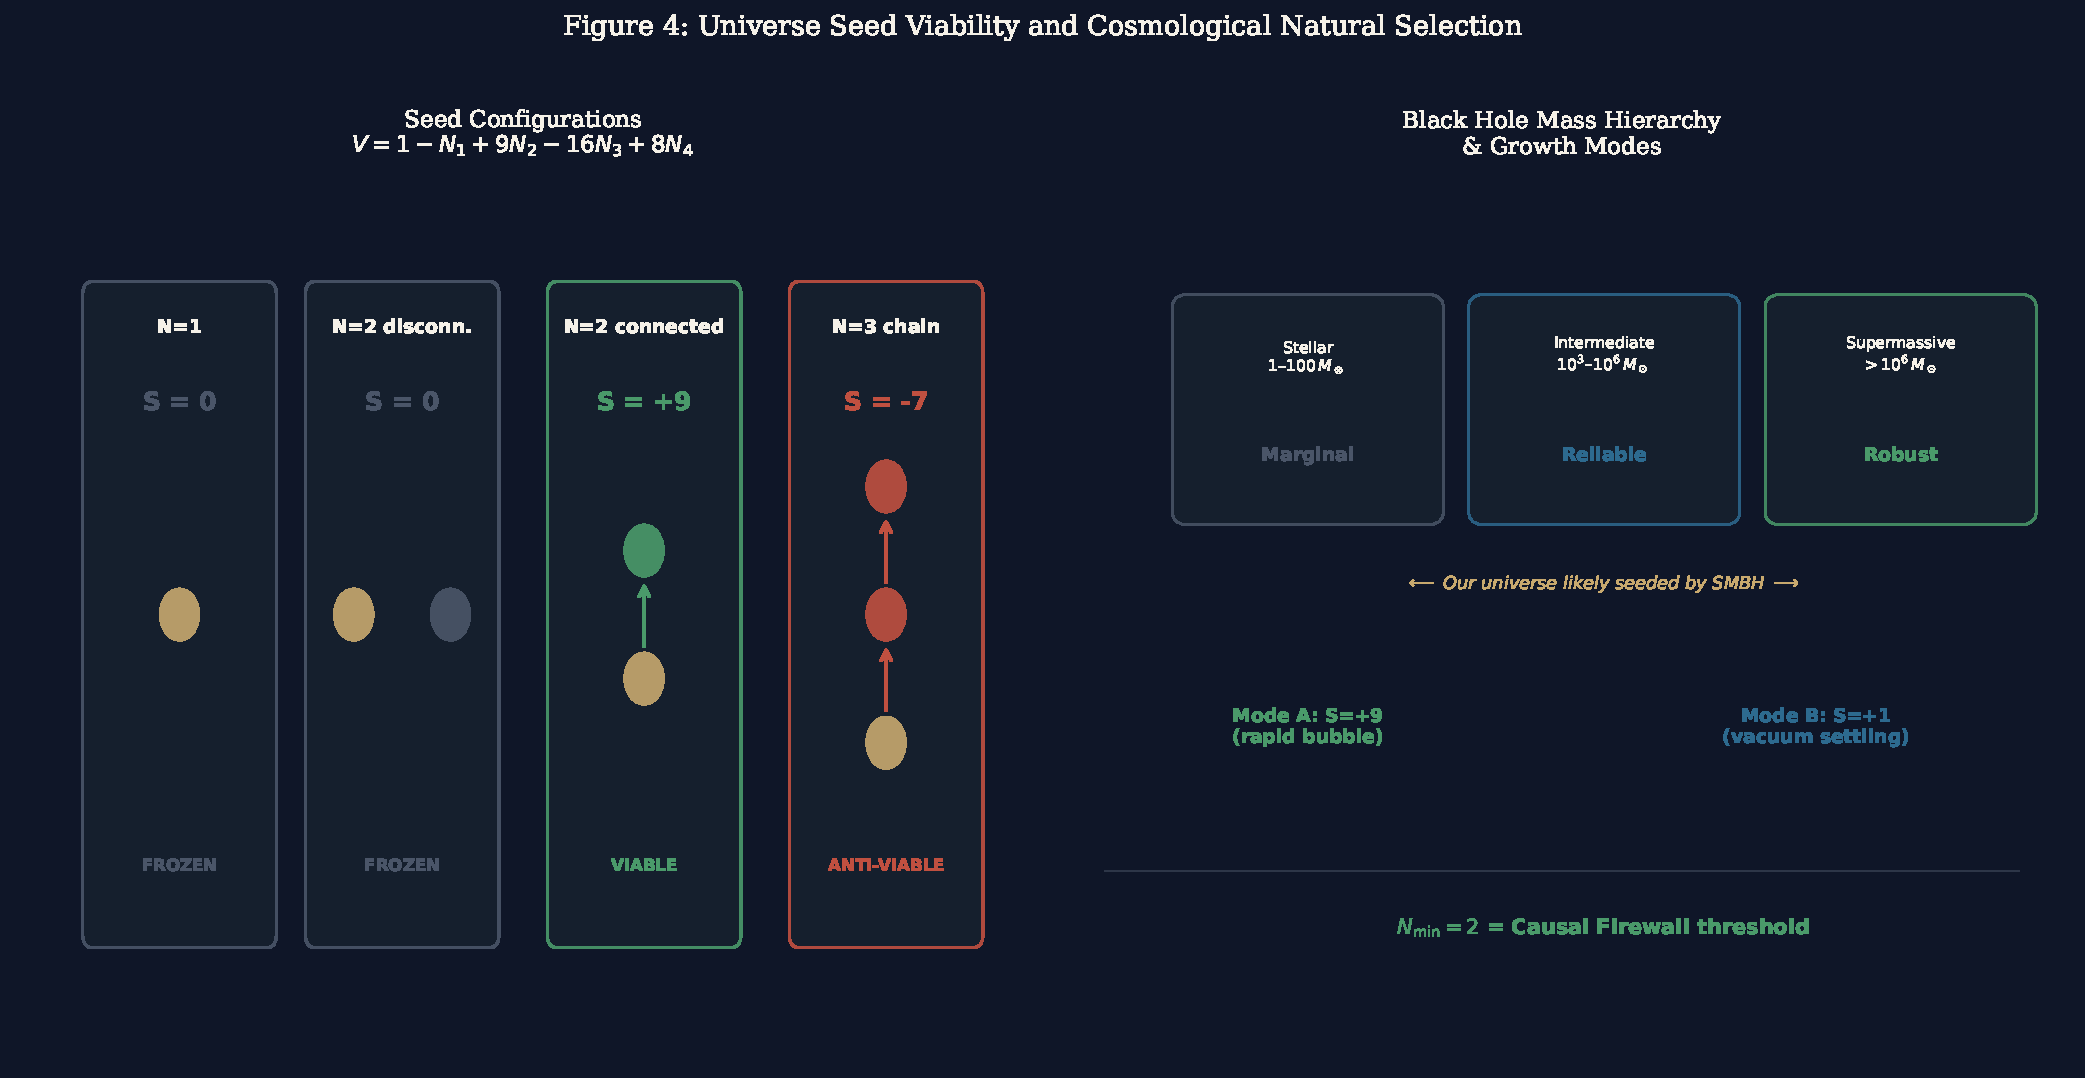
\includegraphics[width=0.88\textwidth]{fig4_seeds}
\caption{Left: Universe seed viability table with BDG action scores.  The $N=2$ connected seed produces $V=+9$ (strongly viable) for the first new vertex.  Right: two stable growth modes (Mode~A rapid expansion, Mode~B vacuum completion); the black hole mass hierarchy; and the $N_{\min}=2$ = Causal Firewall identity.}
\label{fig:seeds}
\end{figure}

\subsection{Frozen and Anti-Viable Seeds}

Understanding why some seeds fail illuminates why $N_{\min}=2$ is the minimum.

\paragraph{$N=1$, $N=2$ disconnected.}  The first new vertex sees no predecessors at depths 1--4: $V=c_0=1>0$.  The vertex actualizes, but subsequent vertices see only depth-1 predecessors ($N_1\geq1$, $N_2=N_3=N_4=0$), giving $V=1-N_1$ which is $\leq0$ for $N_1\geq1$.  The graph grows one vertex and then freezes.

\paragraph{$N=3$ linear chain.}  The BDG coefficient $c_3=-16$ is large and negative.  A three-element chain $v_0\prec v_1\prec v_2$ presents $N_1=1$, $N_2=1$, $N_3=1$ to the next vertex, giving $V=1-1+9-16=-7<0$.  This is anti-viable: the three-chain actively suppresses growth.  The large negative coefficient at depth 3 is the BDG mechanism for preventing three-step chains from dominating; it forces the causal graph to grow in connected, locally dense patterns rather than long chains.

\paragraph{$N=4$ chain (vacuum configuration).}  With $N_1=N_2=N_3=N_4=1$: $V=1-1+9-16+8=+1$.  This is the marginal ``vacuum'' configuration.  It can grow, but barely.  This corresponds to the current cosmological epoch: the universe has expanded to low density, and $V\approx+1$ means exactly one new vertex is accepted for each existing vertex on average.

\subsection{Two Stable Growth Modes}

Simulation of the complete space of vertex placements from the $N=2$ connected seed reveals two coexisting stable growth modes (\statusDR, CB01 and CB02):

\paragraph{Mode~A (parallel chains, rapid expansion).}  Each new vertex connects to both $v_0$ and $v_1$ and to all vertices added so far, maintaining $N_2\geq1$.  The viability $V=+9$ is maintained at each step.  This corresponds to the rapid early universe expansion phase: the causal graph grows exponentially in a highly connected state.

\paragraph{Mode~B (sequential chain, vacuum completion).}  Chain growth completes the 4-chain vacuum configuration.  New vertices connect to the most recent predecessor only, reducing $V$ toward $+1$.  This corresponds to the current epoch: the universe has expanded to low density and the growth rate is approximately constant.

Both modes operate simultaneously in different regions of the causal graph.  The transition from Mode~A to Mode~B corresponds to the exit from the inflationary-like rapid expansion phase into the current matter/dark-energy-dominated epoch.

\subsection{The Black Hole Mass Hierarchy and Seed Viability}

The viability of a universe seed depends on the internal causal structure of the parent black hole at the moment of severance.  Black holes with richer internal causal structure (higher $N_2$ count, indicating more depth-2 connections) produce more viable seeds.

The relevant quantity is the typical $N_2$ value in the black hole interior at severance.  This depends on the black hole's accretion history:

\begin{table}[ht]
\centering
\caption{Black hole mass classes and universe seed viability.}
\label{tab:BH_hierarchy}
\begin{tabular}{p{3.5cm}p{2cm}p{2.5cm}l}
\toprule
Black hole class & Mass range & Typical $N_2$ & Seed viability \\
\midrule
Stellar mass & $1$--$100\,M_\odot$ & $0$--$1$ & Marginal or frozen \\
Intermediate mass & $10^3$--$10^6\,M_\odot$ & $1$--$3$ & Reliably viable \\
Supermassive & $10^6$--$10^{10}\,M_\odot$ & $2$--$5$ & Robustly viable \\
\bottomrule
\end{tabular}
\end{table}

Our universe, with its well-calibrated coupling constants and near-flat geometry, was most likely seeded by a supermassive black hole.  This is consistent with observations:
\begin{itemize}
  \item The measured coupling constants agree with the BDG predictions (Paper~I), indicating the parent universe also operated at $\mu\approx1$.
  \item The spatial flatness ($\Omega\approx1$) is consistent with the Mode~B vacuum configuration ($V\approx+1$) that dominates in large, old black holes.
  \item The baryon asymmetry $\eta\approx6\times10^{-10}$ is an initial condition set at severance.
\end{itemize}

\subsection{Cosmological Natural Selection with Exact Mechanism}

Smolin \cite{Smolin1992} proposed Cosmological Natural Selection (CNS): universes reproduce through black holes and are selected for constants that maximise black hole production.  The proposal was physically compelling but lacked a precise selection mechanism.  RA provides it.

\paragraph{The selection condition.}  A child universe is viable iff its seed satisfies $V>0$.  The BDG condition for $V>0$ from a connected $N=2$ seed: the seed must present $N_2\geq1$ to the first new vertex.  This requires a directed edge between the two seed vertices (otherwise $N_2=0$ and the seed is frozen or marginal).

\paragraph{Fitness of the parent.}  A parent universe produces more viable children if it produces black holes with richer $N_2$ structure (higher depth-2 connectivity in their interiors).  This is favoured by:
\begin{itemize}
  \item More frequent and longer-lived stars (producing stellar-mass black holes).
  \item More efficient galaxy formation (producing supermassive black holes).
  \item Coupling constants that allow rich chemistry and structure formation.
\end{itemize}

\paragraph{Inheritance.}  The BDG integers $(1,-1,9,-16,8)$ are inherited from the parent universe (they are fixed by the four-dimensional geometry of the child universe, which inherits $d=4$ from the parent via the SM closure condition L11 \statusLV).

\paragraph{The D4U02 connection.}  Paper~I proves that $\mu^*\approx1.019$ --- the BDG filter is maximally selective near Planck density.  This means universes that operate at Planck density produce the highest-quality causal graph structure.  The selectivity maximum is itself selected across generations: universes with $\mu\approx1$ produce better seeds, which produce more child universes, which all inherit $\mu\approx1$.

\textbf{CNS in RA has an exact mechanism: the BDG filter $S>0$, operating at every vertex, selects for causal graph structures that maximise viable seed production.  The selection pressure is not an additional hypothesis but a consequence of the BDG dynamics.}

%═══════════════════════════════════════════════════════════════════════════════
\section{Predictions}\label{sec:predictions}
%═══════════════════════════════════════════════════════════════════════════════

\begin{table}[ht]
\centering
\caption{All predictions from Paper~III.}
\label{tab:predictions}
\begin{tabular}{lp{6cm}lp{3.5cm}}
\toprule
ID & Prediction & Status & Experiment \\
\midrule
P02 & $H_0\propto\rho_b^{-1/2}(\hat{n})$; $75.9\,\mathrm{km/s/Mpc}$ at Eridanus & \statusCV & DESI, now \\
P03 & No DM signal below neutrino floor (categorical) & \statusDR & LZ/XENONnT \\
P-III-1 & $\Sigma m_\nu\approx59\,\mathrm{meV}$ (Koide neutrino extension) & conj. & CMB-S4/Euclid \\
P-III-2 & $\theta_{\rm QCD}=0$; no QCD axion & \statusDR & Axion searches \\
P-III-3 & No proton decay at any energy & \statusDR & Proton decay exp. \\
P-III-4 & $a_0^{\rm RA}\approx1.2\times10^{-10}\,\mathrm{m/s}^2$ (no new param.) & \statusAR & Galaxy rotation curves \\
P-III-5 & BH mass hierarchy (supermassive seeds our universe) & \statusDR & Cosmological observations \\
\bottomrule
\end{tabular}
\end{table}

%═══════════════════════════════════════════════════════════════════════════════
\section{Discussion and Open Problems}\label{sec:discussion}
%═══════════════════════════════════════════════════════════════════════════════

\subsection{The Five-in-One Structure}

The five cosmological problems dissolve from the same single ontological commitment.  The cosmological constant is zero because the vacuum does not actualize.  The Hubble tension is an actualization-density gradient.  Dark matter is graph topology.  Boltzmann Brains cannot form because the BDG filter requires causal history.  The Big Bang is a causal severance with minimum viable seed $N_{\min}=2$.

No additional parameters or mechanisms are introduced.  Every result follows from the BDG integers and the LLC.

\subsection{The Baryon Asymmetry}

The observed baryon-to-photon ratio $\eta\approx6\times10^{-10}$ is one of the most precisely measured cosmological parameters.  In standard cosmology, it is explained by leptogenesis or electroweak baryogenesis: mechanisms that generate a baryon excess from an initially baryon-symmetric state.  Both require baryon-number-violating processes, which RA prohibits (baryon number is LLC on winding number, exactly conserved).

In RA, $\eta$ is an initial condition.  The universe was born with a specific baryon-to-photon ratio, set at the causal severance event.  What determines this ratio is an open problem: the LLC boundary conditions at severance nucleation must select a specific value of $\eta$.  This is Open Problem O-III-2.

\subsection{Open Problems}

\paragraph{O-III-1 (Curved Bianchi identity).}  D04 (LLC $\Rightarrow$ Bianchi flat) needs to be extended to curved backgrounds.  The perturbative approach gives the result to $O(\ell_P/R)^2$.

\paragraph{O-III-2 (Baryon asymmetry initial condition).}  Why $\eta=6\times10^{-10}$?  The LLC boundary conditions at causal severance must select this value.  The calculation has not been carried out.

\paragraph{O-III-3 (Dark energy mechanism).}  With $\Lambda=0$, the observed accelerated expansion requires an explanation.  Intrinsic graph growth is the natural candidate but has not been quantified.

\paragraph{O-III-4 ($a_0^{\rm RA}$ complete derivation).}  The geometric factor $f(\text{geometry})$ in Eq.~(\ref{eq:a0_RA}) needs to be computed from the BDG causal diamond structure.  This would make the rotation-curve transition scale a fully derived quantity.

\section*{Acknowledgments}

Developed with AI collaboration (Claude, Anthropic; Gemini, Google).  Lean~4 proofs at \url{https://github.com/jsandeman/Relational-Actualism}.

\bibliographystyle{plain}
\begin{thebibliography}{99}
\bibitem{RA_P1} Sandeman, J.~F. (2026). Paper~I. Zenodo, doi:10.5281/zenodo.19362289.
\bibitem{RA_P2} Sandeman, J.~F. (2026). Paper~II. Zenodo, doi:10.5281/zenodo.19362968.
\bibitem{RA_P4} Sandeman, J.~F. (2026). Paper~IV. Zenodo, doi:10.5281/zenodo.19198224.
\bibitem{Durhuus1995} Durhuus, B., Jonsson, T., and Wheater, J. (1995). \textit{J.\ Stat.\ Phys.}, 78, 827.
\bibitem{Gibbons1977} Gibbons, G.~W., and Hawking, S.~W. (1977). Action integrals and partition functions in quantum gravity. \textit{Phys.\ Rev.~D}, 15, 2752.
\bibitem{Jacobson1995} Jacobson, T. (1995). Thermodynamics of spacetime. \textit{Phys.\ Rev.\ Lett.}, 75, 1260.
\bibitem{Keenan2013} Keenan, R.~C., Barger, A.~J., and Cowie, L.~L. (2013). \textit{ApJ}, 775, 62.
\bibitem{Lovelock1971} Lovelock, D. (1971). The Einstein tensor and its generalizations. \textit{J.\ Math.\ Phys.}, 12, 498.
\bibitem{McGaugh2016} McGaugh, S.~S., Lelli, F., and Schombert, J.~M. (2016). Radial acceleration relation in rotationally supported galaxies. \textit{Phys.\ Rev.\ Lett.}, 117, 201101.
\bibitem{Milgrom1983} Milgrom, M. (1983). A modification of the Newtonian dynamics. \textit{ApJ}, 270, 365.
\bibitem{PDG2024} Particle Data Group (2024). Review of Particle Physics. \textit{PTEP} 2022, 083C01.
\bibitem{Planck2020} Planck Collaboration (2020). Planck 2018 results VI. \textit{A\&A}, 641, A6.
\bibitem{Riess2022} Riess, A.~G.\ et al.\ (2022). \textit{ApJL}, 934, L7.
\bibitem{Smolin1992} Smolin, L. (1992). Did the universe evolve? \textit{CQG}, 9, 173.
\bibitem{Weinberg1964} Weinberg, S. (1964). \textit{Phys.\ Rev.}, 135, B1049.
\end{thebibliography}
\end{document}
